%%%%%%%%%%%%%%%%%%%%%%%%%%%%%%%%%%%%%%%%%%%
%%% DOCUMENT PREAMBLE %%%
\documentclass[12pt]{report}
\usepackage[italian]{babel}

\usepackage[normalem]{ulem}
\useunder{\uline}{\ul}{}
\usepackage{longtable}
\usepackage{url}
\usepackage{placeins}
\usepackage[utf8x]{inputenc}
\usepackage{amsmath}
\usepackage{graphicx}
\graphicspath{{images/}}
\usepackage{parskip}
\usepackage{fancyhdr}
\usepackage{vmargin}
\usepackage{nameref}
\setmarginsrb{3 cm}{2.5 cm}{3 cm}{2.5 cm}{1 cm}{1.5 cm}{1 cm}{1.5 cm}

\title{uCOM}								
% Title
\author{Mazzaglia Pietro}						
% Author

\makeatletter
\let\thetitle\@title
\let\theauthor\@author
\newcommand*{\currentname}{\@currentlabelname}
\makeatother

\pagestyle{fancy}
\fancyhf{}
\lhead{\thetitle}
\rhead{\currentname}
\cfoot{\thepage}


\begin{document}
	
	\huge \textbf{Elaborazione - Iterazione 2}
	
	\renewcommand{\thesection}{\arabic{section}}
	
	\normalsize
	
	%%%%%%%%%%%%%%%%%%%%%%%% PIANIFICAZIONE %%%%%%%%%%%%%%%%%%%%%%

	\section{Introduzione}
	
	Nota la seguente tabella di pianificazione:
	
	
	% Please add the following required packages to your document preamble:
	% \usepackage{graphicx}
	\begin{table}[!htb]
		\centering
		\resizebox{\textwidth}{!}{%
			\begin{tabular}{|l|l|l|}
				\hline
				\textbf{Priorità} & \textbf{Requisiti  (Casi d'uso o funzionalità)}                                                                          & \textbf{Commento}                                                                                                                                                                                                                                \\ \hline
				\textbf{Alta}              & \begin{tabular}[c]{@{}l@{}}\textbf{Invia comunicazione}\\ \\ \textbf{Invia avviso}\\ \\ \textbf{Gestisce utente}\\ \\ \textbf{Effettua accesso}\end{tabular} & \begin{tabular}[c]{@{}l@{}}\textbf{Nucleo della piattaforma, alta frequenza}\\ \\ \textbf{Nucleo della piattaforma, alta frequenza}\\ \\ \textbf{Nucleo della piattaforma, sicurezza}\\ \\ \textbf{Nucleo della piattaforma, sicurezza, coinvolta in tutte le funzioni}\end{tabular} \\ \hline
				Media             & \begin{tabular}[c]{@{}l@{}}Prenota pasto\\ \\ Richiede libro\end{tabular}                                                & \begin{tabular}[c]{@{}l@{}}Frequenza elevata e più parti interessate ma sostituibile\\ \\ Frequenza elevata e più parti interessate ma sostituibile\end{tabular}                                                                                 \\ \hline
				Bassa             & \begin{tabular}[c]{@{}l@{}}Iscrive a un corso\\ \\ Gestisce corso\\ \\ Gestisce iscrizione corso\end{tabular}            & \begin{tabular}[c]{@{}l@{}}Bassa frequenza e sostituibile\\ \\ Bassa frequenza e sostituibile\\ \\ Bassa frequenza e sostituibile \end{tabular}                                                                                                                                                \\ \hline
			\end{tabular}%
		}
	\end{table}
	
	
	Gli obiettivi della seconda iterazione sono:
	\begin{itemize}
		\item Analisi e progettazione, relativamente agli scenari dei casi d'uso \textit{UC7: Invia avviso} e \textit{UC8: Gestisce utente}
		\item Refactoring del codice dell'Iterazione 1 al fine di renderlo testabile con maggiore facilità
		\item Arricchimento dell'implementazione dei casi d'uso dell'Iterazione 1 (UC4 e UC9)
		\item Implementazione caso d'uso \textit{UC8}
	\end{itemize}
	
	Si è scelto di implementare prima il caso d'uso UC8, in quanto UC7 sembra essere simile a UC4, e necessita dunque di uno sforzo di progettazione e implementazione inferiore, che potrà essere svolto nelle prossime iterazioni.
	
	Svolgendo le prime iterazioni è importante elaborare prima le parti più critiche del software e risolvere le problematiche più complesse a monte.	
	
	\newpage
	
	\section{Modello dei casi d'uso}
	
	Seguono l'aggiornamento dell'\textit{UC7} con correzioni e precisazioni rispetto alla fase di Ideazione e la descrizione dettagliata dell'\textit{UC8}.
	
	Inoltre si presentano i \textit{Diagrammi di sequenza di sistema} relativi agli scenari di successo e i \textit{Contratti delle operazioni}.
	
	\subsection{UC7: Invia avviso}

	
\begin{longtable}{|l|l|}
	\hline
	\textbf{Nome caso d'uso}                                                                          & UC7: Invia avviso                                                                                                                                                                                                                                                                                                                                                                                                                                                                                                                                                                                                                                                                                                                                                                                                                                                                                                                                                                                                                                                                                                                                            \\ \hline
	\endfirsthead
	%
	\endhead
	%
	\textbf{Portata}                                                                                  & Piattaforma uCOM                                                                                                                                                                                                                                                                                                                                                                                                                                                                                                                                                                                                                                                                                                                                                                                                                                                                                                                                                                                                                                                                                                                                             \\ \hline
	\textbf{Livello}                                                                                  & Obiettivo utente                                                                                                                                                                                                                                                                                                                                                                                                                                                                                                                                                                                                                                                                                                                                                                                                                                                                                                                                                                                                                                                                                                                                             \\ \hline
	\textbf{Attore primario}                                                                          & Amministratore                                                                                                                                                                                                                                                                                                                                                                                                                                                                                                                                                                                                                                                                                                                                                                                                                                                                                                                                                                                                                                                                                                                                               \\ \hline
	\textbf{\begin{tabular}[c]{@{}l@{}}Parti interessate \\ e Interessi\end{tabular}}                 & \begin{tabular}[c]{@{}l@{}}Amministratore: vuole inviare un avviso relativo\\ alla vita all'interno del Campus\\ \\ Studente: vuole potere ricevere la comunicazione\\  dall'amministrazione\\ \\ Direzione Campus: vuole che la comunicazione \\ avvenga in maniera rapida, sicura e affidabile\end{tabular}                                                                                                                                                                                                                                                                                                                                                                                                                                                                                                                                                                                                                                                                                                                                                                                                                                                \\ \hline
	\textbf{Pre-condizioni}                                                                           & L'Amministratore possiede un account sulla piattaforma.                                                                                                                                                                                                                                                                                                                                                                                                                                                                                                                                                                                                                                                                                                                                                                                                                                                                                                                                                                                                                                                                                                      \\ \hline
	\textbf{Garanzia di successo}                                                                     & L'Amministratore ha ricevuto conferma dell'operazione.                                                                                                                                                                                                                                                                                                                                                                                                                                                                                                                                                                                                                                                                                                                                                                                                                                                                                                                                                                                                                                                                                                       \\ \hline
	\textbf{\begin{tabular}[c]{@{}l@{}}Scenario principale \\ di successo\end{tabular}}               & \begin{tabular}[c]{@{}l@{}}1. L'Amministratore effettua l'accesso\\ 2. L'Amministratore avvia l'operazione di invio dell'avviso.\\ 3. L'Amministratore inserisce titolo e dettagli dell'avviso.\\ 4. L'Amministratore invia l'avviso.\\ 5. Il Sistema elabora l'avviso.\\ 6. Il Sistema conferma la riuscita dell'operazione.\end{tabular}                                                                                                                                                                                                                                                                                                                                                                                                                                                                                                                                                                                                                                                                                                                                                                                                                      \\ \hline
	\textbf{Estensioni}                                                                               & \begin{tabular}[c]{@{}l@{}}*a. In qualsiasi momento.Il Sistema non è in grado di funzionare \\ correttamente in un dato momento.\\ \\ \quad 1) Il Sistema segnala l'impossibilità di eseguire l'azione.\\ \\   \quad  - L'Amministratore riprova a eseguire l'azione dopo un certo \\ periodo di tempo.\\ \\ *b. In qualsiasi momento. Il Sistema entra in uno stato di errore\\ irrisolvibile.\\ \\  \quad   1) Il Sistema termina la sessione, perdendo i dati.\\ \\ \quad    - L'Amministratore deve ricominciare l'operazione.\\ \\ *c. In qualsiasi momento. L'Amministratore \\interrompe l'operazione. \\ \\ \quad 1)Il Sistema termina l'operazione. \\ \\ 3a. L'Amministratore inserisce informazioni non valide.\\ \\  \quad   1) Il Sistema richiede nuova immissione dei dati \\ all'Amministratore.\\ \\ 5a. Il Sistema invia il messaggio a un Servizio Esterno.\\ \\  \quad   1a) Il Servizio Esterno riceve correttamente il messaggio.\\  \\   \quad \quad      2) Il Sistema conferma la riuscita dell'operazione.\\ \\  \quad   1b) Il Servizio Esterno rigetta la richiesta.\\ \\   \quad \quad      - Il Sistema va in errore temporaneo.\\ \\    \quad \quad     - L'Amministratore può ritentare l'operazione dopo un certo\\           periodo di tempo.\\ \\ 5b. Il Sistema gestisce internamente il messaggio.\end{tabular} \\ \hline
	\textbf{Requisiti speciali}                                                                       & \begin{tabular}[c]{@{}l@{}}- L'Amministratore deve poter inserire le informazioni nella \\ lingua di comunicazione del Campus.\end{tabular}                                                                                                                                                                                                                                                                                                                                                                                                                                                                                                                                                                                                                                                                                                                                                                                                                                                                                                                                                                                                                  \\ \hline
	\textbf{\begin{tabular}[c]{@{}l@{}}Elenco delle varianti \\ tecnologiche e dei dati\end{tabular}} & \begin{tabular}[c]{@{}l@{}}3) L'inserimento delle informazioni può avvenire attraverso\\ metodi d'input diversi, come tastiera e mouse o un touchscreen.\\ \\ 5) L'elaborazione di sistema può avvenire internamente o\\ esternamente alla piattaforma uCOM.\end{tabular}                                                                                                                                                                                                                                                                                                                                                                                                                                                                                                                                                                                                                                                                                                                                                                                                                                                                                            \\ \hline
	\textbf{Frequenza di ripetizione}                                                                 & quasi giornaliera                                                                                                                                                                                                                                                                                                                                                                                                                                                                                                                                                                                                                                                                                                                                                                                                                                                                                                                                                                                                                                                                                                                                            \\ \hline
	\textbf{Varie}                                                                                    & \begin{tabular}[c]{@{}l@{}}Si potrebbe prevedere un sistema che permetta l'inserimento\\ offline e l'elaborazione non appena il servizio ritorna disponibile.\\ \\ Si potrebbe integrare il servizio esterno all'interno della\\ piattaforma, piuttosto che inviare esternamente l'avviso  \\ per l'elaborazione.\\ \\ L'avviso viene memorizzato dal Sistema se viene elaborato\\ esternamente?\\ \\ Si possono prevedere meccanismi di recupero dell'istanza in\\ caso di errori gravi.\end{tabular}                                                                                                                                                                                                                                                                                                                                                                                                                                                                                                                                                                                                                                               \\ \hline
\end{longtable}
	

	\subsection{UC8: Gestisce utente}

	Questo caso d'uso è di tipo CRUD (Create Read Update Delete). Ai fini dello sviluppo di una versione di prova di \textit{uCOM} sarà trattato solo uno dei quattro scenari, ovvero quello di Creazione dell'utente. Gli altri scenari saranno considerati come estensioni del caso d'uso.

	% Please add the following required packages to your document preamble:
% \usepackage[normalem]{ulem}
% \useunder{\uline}{\ul}{}
% \usepackage{longtable}
% Note: It may be necessary to compile the document several times to get a multi-page table to line up properly
\begin{longtable}{|l|l|}
	\hline
	\textbf{Nome caso d'uso} & UC8: Gestisce utente \\ \hline
	\endfirsthead
	%
	\endhead
	%
	\textbf{Portata} & Piattaforma uCOM \\ \hline
	\textbf{Livello} & Obiettivo utente (CRUD) \\ \hline
	\textbf{Attore primario} & System Admin \\ \hline
	\textbf{\begin{tabular}[c]{@{}l@{}}Parti interessate \\ e Interessi\end{tabular}} & \begin{tabular}[c]{@{}l@{}}SystemAdmin: vuole poter gestire la creazione di un utente\\ per poter accedere alla piattaforma\\ \\ Direzione Campus: necessita che l'accesso di ogni utente\\ sia verificato, per garantire sicurezza al sistema, e che solo un\\ utente autorizzato, quale il SystemAdmin possa modificare\\ gli utenti che possono accedere al Sistema\end{tabular} \\ \hline
	\textbf{Pre-condizioni} & Il SystemAdmin possiede un account sulla piattaforma \\ \hline
	\textbf{Garanzia di successo} & Un nuovo utente può avere accesso alla piattaforma \\ \hline
	\textbf{\begin{tabular}[c]{@{}l@{}}Scenario principale \\ di successo\end{tabular}} & \begin{tabular}[c]{@{}l@{}}1. Il SystemAdmin effettua l'accesso.\\ 2. Il SystemAdmin avvia la creazione di un utente.\\ 3. Il SystemAdmin inserisce username e ruolo per l'utente.\\ 4. Il SystemAdmin aggiunge l'utente al Sistema.\\ 5. Il Sistema aggiunge l'utente al proprio Registro Utenti.\\ 6. Il Sistema conferma la riuscita dell'operazione.\end{tabular} \\ \hline
	\textbf{Estensioni} & \begin{tabular}[c]{@{}l@{}}*a. In qualsiasi momento.Il Sistema non `e in grado di funzionare\\ correttamente in un dato momento.\\ \\ \quad1) Il Sistema segnala l’impossibilità a di eseguire l’azione. \\ \\ \quad- Il SystemAdmin riprova a eseguire l’azione dopo un certo \\ periodo di tempo.\\ \\ *b. In qualsiasi momento. Il Sistema entra in uno stato di errore \\ irrisolvibile. \\ \\ \quad1) Il Sistema termina la sessione, perdendo i dati. \\ \\ \quad- Il SystemAdmin deve ricominciare l’operazione.\\ \\ *c. In qualsiasi momento. Il SystemAdmin \\ interrompe l’operazione. \\ \\ \quad1) Il Sistema termina l’operazione.\\ \\ 2a. Il SystemAdmin avvia la lettura dei dati di un utente.\\ \\ \quad 1) Il SystemAdmin inserisce l'identificativo dell'utente.\\ \\ \quad 2) Il SystemAdmin richiede la lettura dell'utente.\\ \\ \quad 3) Il Sistema preleva i dati dell'utente richiesto \\ dal Registro Utenti.\\ \\ \quad4) Il Sistema restituisce i dati dell'utente richiesto.\end{tabular} \\ \hline
	\textbf{Estensioni} & \begin{tabular}[c]{@{}l@{}}2b. Il SystemAdmin avvia la modifica di un utente.\\ \\ \quad1) Il SystemAdmin inserisce le informazioni dell'utente\\da modificare.\\ \\ \quad2) Il SystemAdmin modifica l'utente.\\ \\ \quad3) Il Sistema aggiorna l'utente sul RegistroUtenti.\\ \\ \quad4) Il Sistema conferma la riuscita dell'operazione.\\ \\ 2c. Il SystemAdmin avvia l'eliminazione di un utente.\\ \\ \quad1) Il SystemAdmin inserisce le informazioni dell'utente\\  da eliminare.\\ \\ \quad2) Il SystemAdmin elimina l'utente.\\ \\ \quad 3) Il Sistema elimina l'utente dal RegistroUtenti.\\ \\ \quad4) Il Sistema conferma la riuscita dell'operazione.\\ \\ 3a. Il SystemAdmin inserisce informazioni non valide. \\ \\ \quad1) Il Sistema richiede nuova immissione dei dati\\ al SystemAdmin\end{tabular} \\ \hline
	\textbf{Requisiti speciali} & Nessuno \\ \hline
	\textbf{\begin{tabular}[c]{@{}l@{}}Elenco delle varianti \\ tecnologiche e dei dati\end{tabular}} & \begin{tabular}[c]{@{}l@{}}3) L'inserimento delle informazioni può avvenire attraverso\\ metodi d'input diversi, come tastiera e mouse o un touchscreen.\end{tabular} \\ \hline
	\textbf{Frequenza di ripetizione} & frequenza medio-bassa \\ \hline
	\textbf{Varie} & \begin{tabular}[c]{@{}l@{}}Si potrebbero aggiungere nuove informazioni da memorizzare sul\\ Registro Utenti.\end{tabular} \\ \hline
\end{longtable}	
	
	
	\newpage
	
	%%%%%%%%%%%%%% ANALISI ORIENTATA AGLI OGGETTI %%%%%%%%%%%%%%%%%
	
	\section{Modello di dominio}
	
	\subsection{Introduzione}
	
	Sulla base dei casi d'uso finora analizzati (UC7 e UC8) sono state identificate le seguenti classi concettuali:
	\begin{itemize}
		\item \textbf{Avviso}
		\item \textbf{Amministratore}		
		\item \textbf{SystemAdmin}
		\item \textbf{Registro Utenti}
	\end{itemize}

	Tenendo conto di associazioni e attributi, a partire dallo schema dell'Iterazione 1, è stato ricavato il seguente Modello di Dominio:
	
	\begin{center}	
	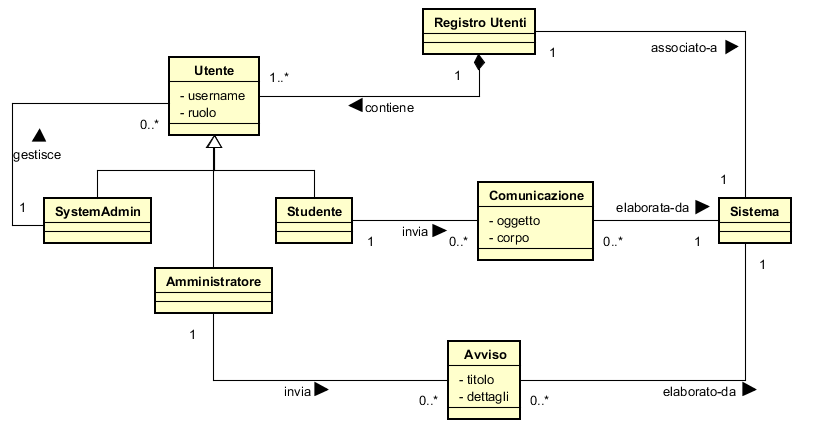
\includegraphics{./images/domain-I2.png}
	\end{center}
	
	I dettagli relativi alle classi sono stati inseriti nel \textbf{Glossario}.
	
	\newpage
	
	\section{Diagrammi di sequenza di sistema e contratti delle operazioni}
	
	I diagramma di sequenza di sistema mostrano gli eventi di I/O del sistema \textit{uCOM}, descrivendo in maniera chiara le interazioni tra attori e sistema.
	
	\subsection{UC7: Invia avviso}
	\begin{center}
		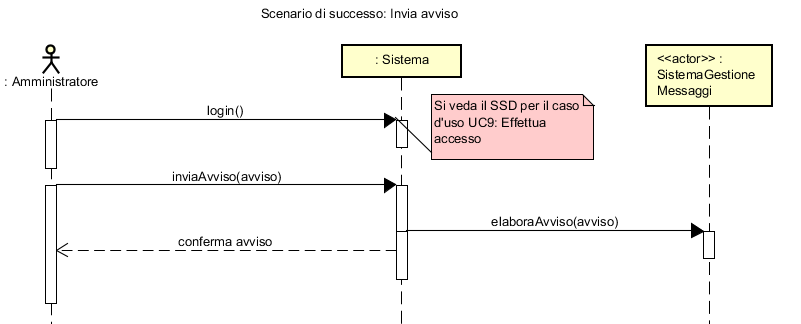
\includegraphics{./images/SSD_UC7.png}
	\end{center}
	
	\newpage	
		
	\subsection{UC8: Gestisce utente}
	
	\begin{center}
		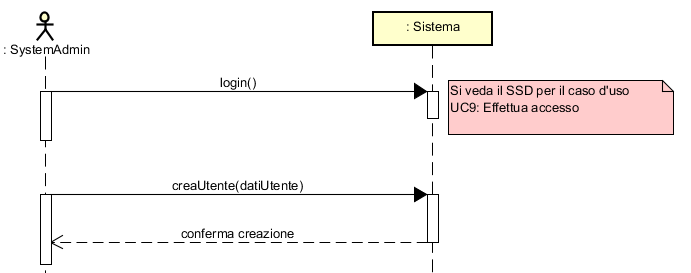
\includegraphics{./images/SSD_UC8.png}
	\end{center}

		%%%%%%% CONTRATTI
	
	\noindent\fbox{%
		\parbox{\textwidth}{%
			\large \textbf{Contratto CO1: creaUtente}\\
			
			\normalsize
			\textbf{Operazione:} \quad \quad creaUtente(datiUtente)\\
			\textbf{Riferimenti:} \quad \quad Caso d'uso: Gestisce utente\\
			\textbf{Pre-condizioni:} \quad - Il Sistema è stato avviato.\\
			.\quad\quad\quad\quad\quad\quad\quad\quad\quad - Il SystemAdmin ha inserito i datiUtente\\ 
			\textbf{Post-condizioni:} \quad - Viene associata una voce del Registro Utenti \\
			.\quad\quad\quad\quad\quad\quad\quad\quad\quad ai datiUtente inseriti
		}%
	}
	
	
	
	%%%%%%%%%%%% PROGETTAZIONE
	\newpage
	
	
	\section{Diagrammi di sequenza}
	
	I diagrammi di sequenza permettono di iniziare a progettare il software, partendo dall'analisi già effettuata. Essi mettono in evidenza le interazioni tra entità che sono già ottime candidate per diventari classi della programmazione orientata ad oggetti.
	
	\subsection{UC7: Invia avviso}
	\begin{center}
		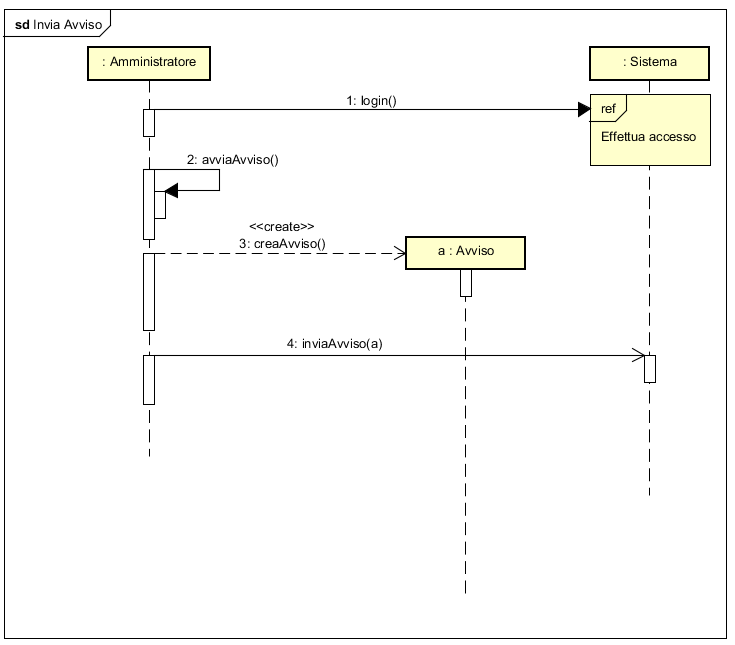
\includegraphics{./images/InviaAvviso.png}
	\end{center}
	
	\subsection{UC7: Elabora avviso}
	\begin{center}
		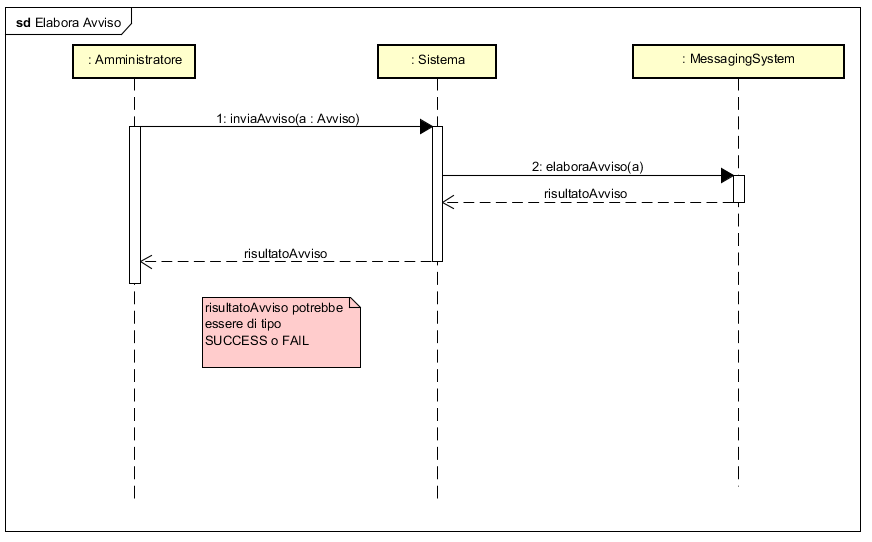
\includegraphics[scale = 0.8]{./images/ElaboraAvviso.png}
	\end{center}

	\subsection{UC8: Aggiungi utente}
	\begin{center}
		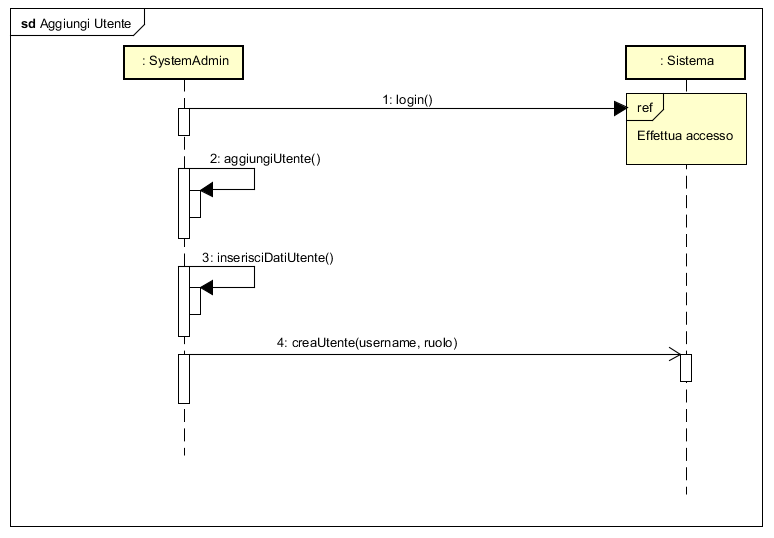
\includegraphics{./images/AggiungiUtente.png}
	\end{center}
		
	\subsection{UC8: Crea utente}
	\begin{center}
		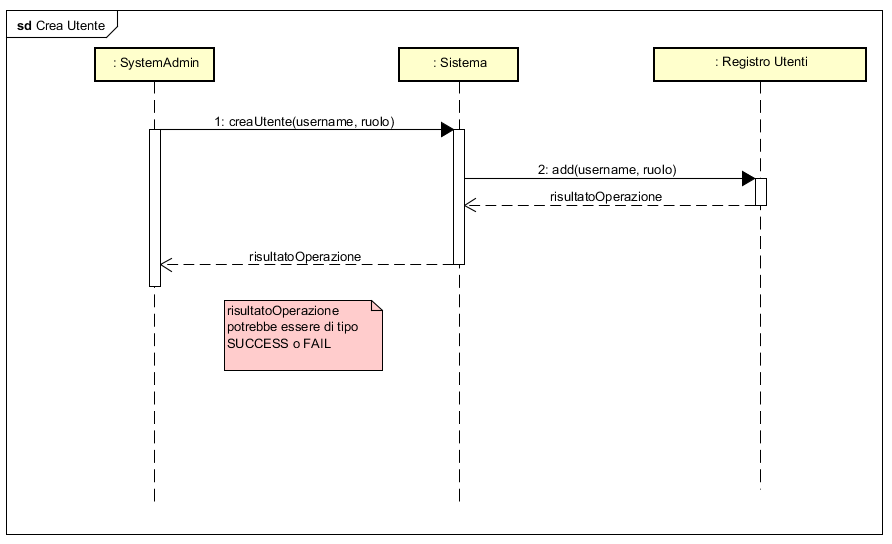
\includegraphics[scale=0.8]{./images/CreaUtente.png}
	\end{center}


	\newpage
	
	\section{Diagrammi delle classi e implementazione}
	
	Il Diagramma delle classi che segue è il risultato di un processo di raffinazione, ottenuto applicando pattern GRASP e alcuni Design Pattern [GOF], a partire dagli elaborati dell'analisi e della progettazione finora svolte.
	
	La sua stesura, laddove l'implementazione è stata avviata, è avvenuta in maniera quasi parallela alla programmazione, per evidenziare fin da subito i punti critici e le difficoltà nella traduzione del diagramma in codice Java.	
	
	\begin{center}
				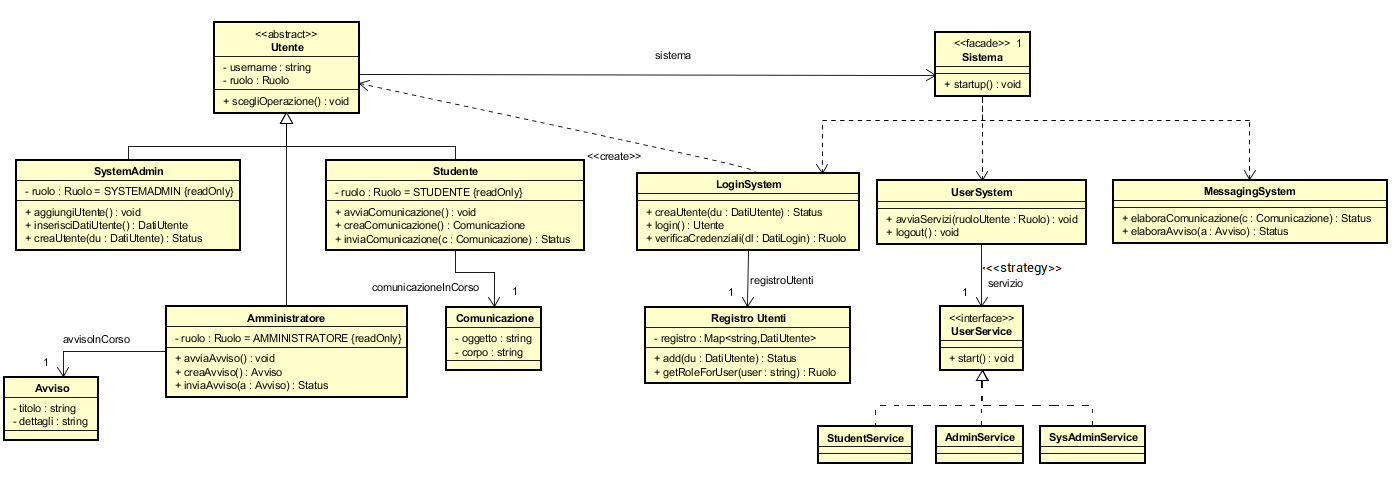
\includegraphics[scale= 0.6]{./images/DCD-I2.png}
	\end{center}

	Alla fine di questa iterazione sono stati implementati quattro casi d'uso completi, con buona parte delle estensioni disponibili, oltre agli scenari di successo.
	
	L'implementazione è avvenuta più rapidamente del previsto, grazie alla larga riusabilità del codice, dunque si è deciso di procedere anche all'implementazione del caso d'uso \textit{UC7} (pressochè identico all'UC4, ma dal punto di vista di un Amministratore, piuttosto che di uno Studente), che si intendeva inizialmente trascurare.
	
	Si noti che il software presenta ancora molti limiti, tra cui una gestione degli errori poco precisa nel notificare gli errori all'utente e la mancanza di un \textit{Controller} che separi il dominio dall'interfaccia utente (possibile implementazione futura del pattern architetturale MVC).
	
	Tuttavia alcune di queste problematiche non sono ad alta priorità al momento, e verranno trattate nelle future iterazioni.

	\newpage
	
	%%%%%%%%%%%% TESTING
	
	\section{Testing}
	
	Il codice si presta adesso a un maggior numero di test.
	
	Sono stati scritti più di una decina di test che verifichino il funzionamento dei metodi delle classi \textit{LoginSystem}, \textit{MessagingSystem}, \textit{RegistroUtenti} e \textit{UserSystem}.
	
	Per la suite di test a scatola nera sono stati scelti casi di uso normale (scenari di successo) e casi estremi, utilizzando input scelti in maniera specifica per il singolo test.
	
	Il resto del codice è stato testato manualmente cercando di coprire tutti i cammini percorribili.
	
	Con i test della suite JUnit si è raggiunta una copertura del 46\% del codice. Con i test manuali si è invece superato il 90\% di copertura.
	
	Nonostante ciò è possibile che il software celi ancora diversi errori, dovuti a valori di I/O errati (non ancora intercettati) o errori di riferimento ai dati. 
	
	
	
	
\end{document}